%% This is an input file.  It cannot be compiled by itself unless you uncomment
%% the next give lines, and then put `\end{document}` at the bottom of the file.
%% \documentclass{amsart}
%% \usepackage{graphicx}
%% \usepackage{tikz}
%% \usepackage{url}
%% \begin{document}

\noindent {\bf Example diagrams for maps}\\

There's a ton of info on the interweb about creating diagrams like the ones in
this document.  Here are some nice guides with other great examples:
\begin{itemize}

\item 
{\footnotesize
  \url{https://pdp7.org/blog/2011/02/how-to-draw-commutative-diagrams-in-latex-with-tikz/}}
(used for example in Figure~\ref{fig:3})

\item {\footnotesize \url{http://www.jmilne.org/not/Mtikz.pdf}}

\item 
{\footnotesize
  \url{http://texdoc.net/texmf-dist/doc/latex/tikz-cd/tikz-cd-doc.pdf}}

\end{itemize}


Most of the figures shown here use the following tikzpicture options:
{\small
\begin{verbatim}
[node distance=2cm, auto, scale=2]
\end{verbatim}}
\noindent Some or all of these option values could have been set once and for
all at the top of the document using a command like 
{\small
\begin{verbatim}
\tikzset{node distance=2cm, auto, scale=2}
\end{verbatim}}
\noindent I chose not to do this here in case someone wants to extract just one of these
figures and insert it into their document.


%% ------------- Fig 1 ---------------
\begin{figure}[h]
  \caption{some bijections and a commutative diagram}
  %% Fig 1 (left)
  \begin{tikzpicture}[node distance=2cm, auto, scale=2]
    \node (1) at (0,0)  {$1$};
    \node (2) at (1,0)  {$2$};
    \node (3) at (1,1)  {$3$};
    \node (4) at (0,1)  {$4$};
    \draw[<->] (1) -- (2)  node[pos=.5,below] {$f$};
    \draw[<->] (2) -- (3)  node[pos=.5,right] {$g$};
    \draw[<->] (3) -- (4)  node[pos=.5,above] {$f$};
    \draw[<->] (4) -- (1)  node[pos=.5,left] {$g$};
  \end{tikzpicture}
  \hskip1cm
  %% -------------
  %% Fig 1 (right)
  \begin{tikzpicture}[node distance=2cm, auto, scale=2]
    \node (00) at (0,0)  {$b$};
    \node (10) at (1,0)  {$b$};
    \node (11) at (1,1)  {$b$};
    \node (01) at (0,1)  {$a$};
    \node (middle) at (0.5,0.5)  {$\circlearrowleft$};
    \draw[->] (00) -- (10)  node[pos=.5,below] {$1$};
    \draw[->] (01) -- (00)  node[pos=.5,left] {$f$};
    \draw[->] (01) -- (11)  node[pos=.5,above] {$f$};
    \draw[->] (11) -- (10)  node[pos=.5,right] {$1$};
  \end{tikzpicture}
\end{figure}


%% ------------- Fig 2 ---------------
\begin{figure}[h]
  \caption{more commutative diagrams}
  %% Fig 2 (left)
  \begin{tikzpicture}[node distance=2cm, auto, scale=2]
    \node (00) at (0,0)  {$b$};
    \node (10) at (1,0)  {$b$};
    \node (11) at (1,1)  {$b$};
    \node (01) at (0,1)  {$a$};
    \node (2m1) at (2,-1)  {$c$};
    \draw[->] (00) -- (10)  node[pos=.5,below] {$1$};
    \draw[->] (01) -- (00)  node[pos=.5,left] {$f$};
    \draw[->] (01) -- (11)  node[pos=.5,above] {$f$};
    \draw[->] (11) -- (10)  node[pos=.5,right] {$1$};
    \draw[->] (00) -- (2m1)  node[pos=.5,below] {$v$};
    \draw[dashed,->] (10) -- (2m1)  node[pos=.5,below] {$r$};
    \draw[->] (11) -- (2m1)  node[pos=.5,above] {$u$};
  \end{tikzpicture}
  \hskip1cm
  %% -------------
  %% Fig 2 (right)
  \begin{tikzpicture}[node distance=2cm, auto, scale=2]
    \node (00) at (0,0)  {$b$};
    \node (10) at (1,0)  {$b$};
    \node (11) at (1,1)  {$b$};
    \node (01) at (0,1)  {$a$};
    \node (2m1) at (2,-1)  {$c$};
    \draw[->] (00) -- (10)  node[pos=.5,below] {$1$};
    \draw[->] (01) -- (00)  node[pos=.5,left] {$f$};
    \draw[->] (01) -- (11)  node[pos=.5,above] {$f$};
    \draw[->] (11) -- (10)  node[pos=.5,right] {$1$};
    \draw[->,bend right] (00) to node {$v$} (2m1);
    \draw[dashed,->] (10) -- (2m1)  node[pos=.5,below] {$r$};
    \draw[->,bend left] (11) to node {$u$} (2m1);
  \end{tikzpicture}
\end{figure}



%% ------------- Fig 3 ---------------
\begin{figure}[h]
  \caption{created using reference nodes without specifying any coordinates}
  \label{fig:3}
  %% Fig 3 (left)
  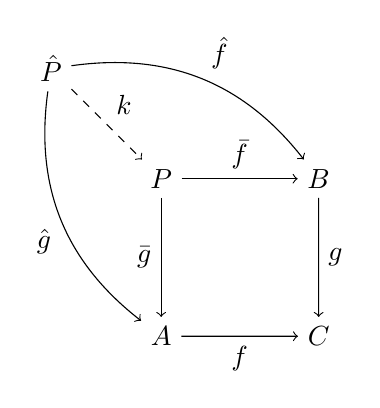
\begin{tikzpicture}[node distance=2cm, auto, scale=1.5]
    \node (P) {$P$};
    \node (B) [right of=P] {$B$};
    \node (A) [below of=P] {$A$};
    \node (C) [below of=B] {$C$};
    \node (P1) [node distance=1.4cm, left of=P, above of=P] {$\hat{P}$};
    \draw[->] (P) to node {$\bar{f}$} (B);
    \draw[->] (P) to node [swap] {$\bar{g}$} (A);
    \draw[->] (A) to node [swap] {$f$} (C);
    \draw[->] (B) to node {$g$} (C);
    \draw[->, bend right] (P1) to node [swap] {$\hat{g}$} (A);
    \draw[->, bend left] (P1) to node {$\hat{f}$} (B);
    \draw[->, dashed] (P1) to node {$k$} (P);
  \end{tikzpicture}
\end{figure}

%% \end{document}
